%%%%%%%%%%%%%%%%%%%%%%%%%%%%%%%%%%%%%%%%%%%%%%%%%%%%%%%%%%%%%%%%%%%%%%%%
% Preamble
%%%%%%%%%%%%%%%%%%%%%%%%%%%%%%%%%%%%%%%%%%%%%%%%%%%%%%%%%%%%%%%%%%%%%%%%
\documentclass[12pt]{article}
%
% Packages and other includes
% Pagination
\usepackage[letterpaper, margin=1in]{geometry}
%
% Graphics, floats, tables
\usepackage{graphicx, color, float, array}
\graphicspath{{image/}}
%
% Fonts
\usepackage[T1]{fontenc} % best for Western European languages
\usepackage{lmodern} % Latin Modern instead of CM
\usepackage{textcomp} % required to get special symbols
%
% Math
\usepackage{amsmath, amssymb}
\usepackage{enumerate}
\usepackage{braket}
% 
% Hyperlinks
\usepackage[colorlinks,linkcolor={red},citecolor={blue},
urlcolor={blue}]{hyperref} 
%
% Definitions and settings
% Paragraph indent and spacing
\setlength{\parskip}{0.4\baselineskip}
\setlength{\parindent}{0in}
%
% Math mode version of "r" column type (requires array package)
\newcolumntype{R}{>{$}r<{$}}
% Title, authors, date
\title{\textbf{Extra Practice: Ch 6 Materials}}
\date{Oct 12, 2022}

\begin{document}

\maketitle 

\textbf{Conservation of Energy}

1) Suppose a system is in thermal equilibrium with a heat bath. If the temperature
of the heat bath increases, describe in words and/or illustrations what happens to
the temperature of the system.

% The temperature of the system increases since the heat bath increases.
% 
%\begin{center}
%  \includegraphics[scale=0.3]{therm_equil.png}
%\end{center}

2) Consider two isolated systems illustrated below. One system (left) is at $100^\circ\text{C}$
and the other (right) is at room temperature of $20^\circ\text{C}$. The isolated systems are allowed
to come into contact reaching thermal equilibrium and without losing energy to the surrounding.
What is the final temperature? Describe in words and/or illustrations what happened.

\begin{center}
  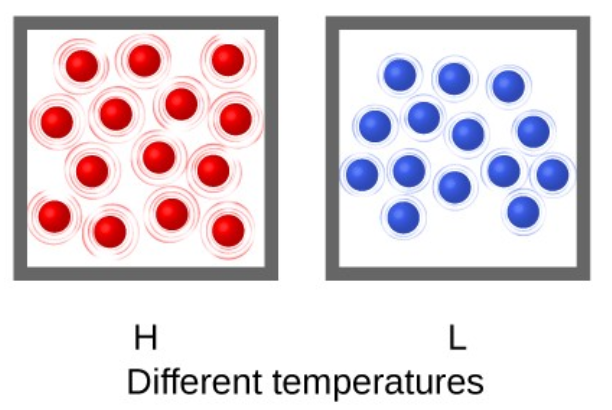
\includegraphics[scale=0.25]{isolated_sys.png}
\end{center}

% 60C is the final temperature; heat move from hot to cold

3) A kilogram of aluminum metal and a kilogram of water are each warmed to 75 °C and placed
in two identical insulated containers. One hour later, the two containers are opened, and
the temperature of each substance is measured. The aluminumvhas cooled to 35 °C, while the
water has cooled only to 66 °C. Explain this difference.

\textbf{Calorimeter}

4) Potassium perchlorate is used as an oxidizer in fireworkds. Calculate the heat
required to raise the temperature of 10.0g of potassium perchlorate from $25^\circ$C
to an ignition temperature of $900.^\circ$C. The specific heat capcity of potassium
perchlorate is $0.8111$ J/($^\circ$C g).

\textbf{Heat Capacity}

5) Calculate the heat that must be supplied to a 500.0g copper kettle containing 400.0g of
water to raise its temperature from 22.0$^\circ$C to the boiling point of water 100.0$^\circ$C.
What percentage of the heat is used to raise the temperature of the water? Heat capacity of
copper is 0.38 J/($^\circ$C g) and water is 4.184 J/($^\circ$C g).

% 1.4 x 10^2 kJ and 90%

\end{document}
